\documentclass{standalone}
% Rare-library spot check (Tier A is whole-tree enumeration; this composite
% only needs a regression signal): spy + mindmap + decorations.footprints +
% shapes.callouts + patterns.meta, all five in one tikzpicture. The mindmap
% library's level styles default to \large/\small, which would request the
% cmr12/cmr9 fonts the closure does not ship (fmt-preload rule) — sizes
% are pinned to \normalsize for the same reason as the fonts figure.
\usepackage{tikz}
\usetikzlibrary{spy,mindmap,decorations.footprints,shapes.callouts,patterns.meta}
\begin{document}
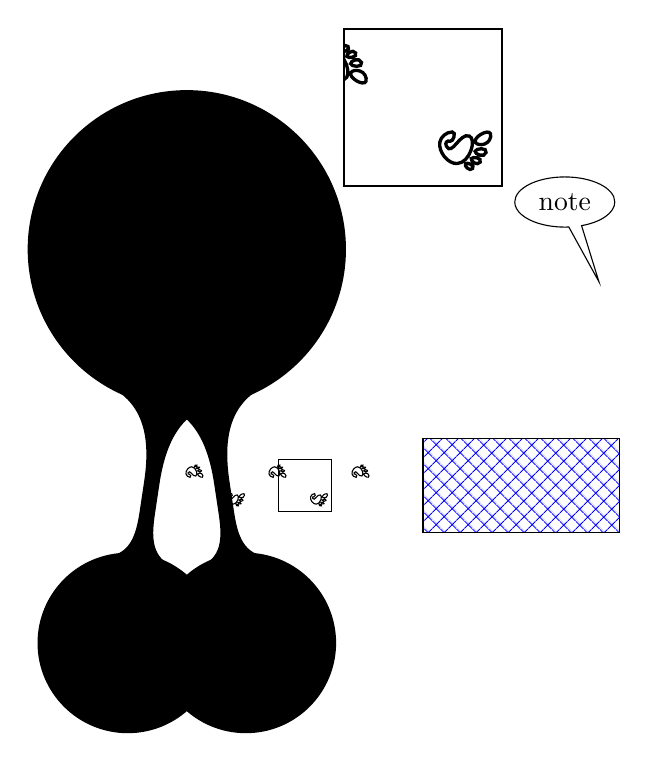
\begin{tikzpicture}[spy using outlines={rectangle, magnification=3, size=2cm}]
\tikzset{root concept/.append style={font=\normalsize}}
\begin{scope}[mindmap, every node/.style={concept, font=\normalsize}]
  \node[root concept] at (0,0) {root}
    child { node {a} }
    child { node {b} };
\end{scope}
\draw[decorate, decoration={footprints, foot length=6pt, foot of=gnome}, line cap=round]
  (0,-3) -- (3,-3);
\node[ellipse callout, draw, callout relative pointer={(0.3,-0.7)}]
  at (4.8,0.6) {note};
\draw[pattern={Hatch[angle=45,distance=4pt]}, pattern color=blue]
  (3,-3.6) rectangle (5.5,-2.4);
\spy on (1.5,-3) in node [right] at (2,1.8);
\end{tikzpicture}
\end{document}
